\documentclass[jou]{apa6}

\usepackage[american]{babel}

\usepackage{csquotes}
\usepackage[style=apa,sortcites=true,sorting=nyt,backend=biber]{biblatex}
\DeclareLanguageMapping{american}{american-apa}
\addbibresource{bibliography.bib}


%%%%%%%%%%%%%%%%%%%%%%%%%%%%%%%%%%%%%%%%
%% Discrete Structures
%% The start of RBS stuff
%%%%%%%%%%%%%%%%%%%%%%%%%%%%%%%%%%%%%%%%

% Working internal and external links in PDF
\usepackage{hyperref}
% Extra math symbols in LaTeX
\usepackage{amsmath}
\usepackage{gensymb}
\usepackage{amssymb}
% Enumerations with (a), (b), etc.
\usepackage{enumerate}
\usepackage{xcolor}

\let\OLDitemize\itemize
\renewcommand\itemize{\OLDitemize\addtolength{\itemsep}{-6pt}}

\usepackage{etoolbox}
\makeatletter
\preto{\@verbatim}{\topsep=3pt \partopsep=3pt }
\makeatother

% These sizes redefine APA for A4 paper size
\oddsidemargin 0.0in
\evensidemargin 0.0in
\textwidth 6.27in
\headheight 1.0in
\topmargin -24pt
\headheight 12pt
\headsep 12pt
\textheight 9.19in



\title{Sample Quiz 8}
\author{Discrete Structures, Spring 2020}
\affiliation{RBS}

\leftheader{Discrete Sample Quiz 8}

\abstract{%
}

%\keywords{}

\setlength\parindent{0pt}

\begin{document}

%\thispagestyle{empty}

\twocolumn
\section{Quiz 9: Advanced Counting}

\vspace{10pt}
{\bf Question 1.} 
You have a rectangular chocolate bar of $2 \times n$ squares. 
Denote by $a(n)$ the ways how you can divide the chocolate bar into 
little dominoes (rectangles $1 \times 2$). 
For example, $a(1) = 1$ and $a(2) = 2$. 
Figure~\ref{fig:domino-tiling} shows a possible tiling for 
the rectangle $2 \times n$, where $n=8$.

\begin{figure}[!htb]
\center{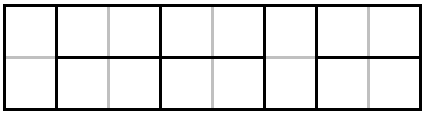
\includegraphics[width=2in]{quiz-09/domino-tiling.png}}
\caption{\label{fig:domino-tiling} Domino Tiling.}
\end{figure}


In your answer write the recurrent expression of {\tt a(n)} (express it through the previous members
of the sequence: {\tt a(n-1),...}).

{\em Note.} Assume that all the little
chocolate squares are distinguishable; the cuts that differ by 
some symmetry (rotation or flip of the chocolate bar) are considered to be different.


\vspace{10pt}
{\bf Question 2.}
Somebody wants to find out, in how many ways it is possible to pay \$15 in a vending machine, using 
\$1 coins, \$1 bills, \$2 bills and \$5 bills, where the order, how you insert them into the machine matters.

In your answer write an integer number.

{\em Note.} In order to solve this, you probably want to define a 
recurrent sequence for $b_n$ and 
find $b_{15}$. People sometimes use characteristic functions for such problems as well:
see \url{https://bit.ly/2Qu4Re4}. Then they can solve some variations of this
problem (what happens, if you have limited number of \$5 bills, etc.), but they need to use
infinite power series and other calculus techniques.

\vspace{10pt}
{\bf Question 3.}
Consider a recurrent sequence: 
$$\left\{ \begin{array}{l}
a_0 = 0,\\
a_1 = 1, \\
a_n = 2a_{n-1} + 2a_{n-2},\;n\geq 2.\\
\end{array} \right.$$
Find both roots of the characteristic equation $r_1,r_2$. 

In you answer write two real numbers, round them to the nearest thousandth.


\vspace{10pt}
{\bf Question 4}
There is a sequence $a(n)$ such that $a(0) = 0$, $a(1) = 0$, $a(2)=1$, but its
characteristic equation is $(r-1)^2(r-2) = 0$. (See \url{https://bit.ly/3a72Ps0} where
the characteristic equations with repeated roots are explained.)
Find the value $a(8)$.

In your answer write a number. 


\vspace{10pt}
{\bf Question 5} 
Write the following expression:\\
{\tt ((A / (B - (C + D))) * E) - (F + (G + H))}\\
in prefix (Polish) notation and also in the postfix (reverse-Polish) notation. 

In your answer separate both expressions with a comma.



\vspace{10pt}
{\bf Question 6} 
Find the number of ways to parenthesize the following expression:\\
{\tt A / B - C + D * E - F + G + H}\\
You should not assume any associativity for the operations.
For example {\tt (F + G) + H} and {\tt F + (G + H)} are two 
different ways to insert parentheses. On the other hand
{\tt (F + G) + H} and {\tt ((F + (G)) + H)} is the same way, since 
the order of execution in both is the same.

In your answer write an integer number.


\vspace{10pt}
{\bf Question 7.} 
Suppose $f(n) = 3f(n/3) + 2n$, $f(1) = 1$. Find $f(3^8)$.

In your answer write an integer number.





\newpage

\subsection{Answers}

\vspace{4pt}
{\bf Question 1.} Answer: {\tt a(n)=a(n-1)+a(n-2)}\\
Notice that the leftmost two squares in the $2 \times n$ 
rectangle can be filled in two different ways:\\
{\bf Alternative 1:} They can be filled by a single vertical domino. 
In this case the remaining rectangle $2 \times (n-1)$ can be 
filled in $a(n-1)$ ways.\\
{\bf Alternative 2:} They can be filled by two horizontal dominoes.
In this case the remaining rectangle $2 \times (n-2)$ can be filled
in $a(n-2)$ ways.\\
The total number of ways is obtained by adding $a(n-1)$ and $a(n-2)$.

{\em Note.} The sequence $a(n)$ is a shifted Fibonacci sequence. 
We can easily verify that $a(n) = F_{n+1}$ for $n \geq 0$.
(We define $F_0 = 0$, $F_1 = 1$ and $F_{n} = F_{n-1} + F_{n-2}$ 
is the regular Fibonacci sequence.)

\vspace{6pt}
{\bf Question 2.} Answer: {\tt 527383}\\
Let us define the sequence $b_n$ (in how many ways you can 
insert \$1 coins, \$1 bills, \$2 bills and \$5 bills into a vending 
machine so that it adds up to $n$ dollars).\\
But before that we consider a simpler sequence $a_n$ (in how many ways you can 
insert \$1 coins, \$1 bills, \$2 bills into a vending machine to pay $n$ dollars \textendash{}
i.e.\ you do not use \$5 bills at all). 

Sequence $a_n$ was already discussed in the {\em Sample Quiz 9}, Problem 2. 
It is defined as a recurrent sequence:
$$\left\{ \begin{array}{l}
a_1 = 2, \\
a_2 = 5, \\
a_{n} = 2a_{n-1} + a_{n-2},\;n \geq 3.\\
\end{array} \right.$$

If you wish, you can also define $a_0 = 1$ (there is exactly one way how to pay \$0 \textendash{}
use zero instances of every coin and bill). Compute the initial members of this sequence:
$$(a_1,a_2,a_3,a_4) = (2,5,12,29).$$

Notice that the sequence $b_n$ (where we also allow \$5 bills) would have exactly same 
members up to $b_4$ (because sums up to $4$ dollars cannot use any \$5 bills anyway).
Further members of $b_n$ can be defined recursively:
$$\left\{ \begin{array}{l}
b_0 = 1,\\
b_1 = 2,\\
b_2 = 5,\\
b_3 = 12,\\
b_4 = 29,\\
b_n = 2b_{n-1} + b_{n-2} + b_{n-5},\;n \geq 5.\\
\end{array} \right.$$

The last (recurrent) line means that $b_n$ ($n \geq 5$) is a total of four different kinds of sequences:
\begin{itemize}
\item Some sequences start from a \$1 coin; the rest is paid in $b_{n-1}$ different ways.
\item Some sequences start from a \$1 bill; the rest is paid in $b_{n-1}$ different ways.
\item Some sequences start from a \$2 bill; the rest is paid in $b_{n-2}$ different ways.
\item Some sequences start from a \$5 bill; the rest is paid in $b_{n-5}$ different ways.
\end{itemize}

Here are the first members $b_0,\ldots,b_{15}$ of this sequence:

$1,\; 2,\; 5,\; 12,\; 29,\; 71,\; 173,\; 422,\; 1029,\; 2509,\; 6118,$
$14918,\; 36376,\; 88699,\; 216283,\; 527383$.




\vspace{6pt}
{\bf Question 3.} Answer:\\ {\tt 2.732,-0.732} or 
{\tt -0.732,2.732} \\
The characteristic equation is 
$$r^2 - 2r - 2 = 0.$$
And the roots of this square equation are 
$r_{1,2} = 1 \pm \sqrt{3}$.
By rounding them to the nearest thousandth, we get
the answer. 

{\em Note.} By the way, we can also 
find the formula for $a_n$. (See {\em Sample Quiz 9}, 
Problem 3, {\bf (B)}.)

\vspace{6pt}
{\bf Question 4} Answer: {\tt 247}\\
Rewrite the characteristic equation:
\begin{align}
(r-1)^2(r-2) & = (r^2 - 2r + 1)(r-2) = \nonumber \\
 & = r^3 - 2r^2 + r - 2r^2 + 4r - 2 = \nonumber \\
 & = r^3 - 4r^2 + 5r - 2 = 0. \nonumber
\end{align}
We can restore the recurrent relationship from here: 
$$a_{n} = 4a_{n-1} - 5a_{n-2} + 2a_{n-3}.$$

\begin{tabular}{|c|r|r|r|r|r|r|r|r|r|} \hline
$n$   & 0 & 1 & 2 & 3 & 4  & 5  & 6  & 7   & 8 \\ \hline
$a_n$ & 0 & 0 & 1 & 4 & 11 & 26 & 57 & 120 & 247 \\ \hline
\end{tabular}


\vspace{6pt}
{\bf Question 5} Answer:\\ 
{\tt -*/A-B+CDE+F+GH, ABCD+-/E*FGH++-}\\
In order to transform infix notation into postfix notation
we can do this step by step. We start with the last/outermost operation
(minus in our case). And leave both subexpressions in 
the infix form. Then we find the last/outermost operation 
the subexpressions and so on.

{\tt ((A/(B-(C+D)))*E) - (F+(G+H))}\\
{\tt \textcolor{red}{-} ((A/(B-(C+D)))*E) (F+(G+H))}\\
{\tt \textcolor{red}{- *} (A/(B-(C+D))) E (F+(G+H))}\\
{\tt \textcolor{red}{- * /} A (B-(C+D)) E (F+(G+H))}\\
{\tt \textcolor{red}{- * /} A \textcolor{red}{-} B (C+D) E (F+(G+H))}\\
{\tt \textcolor{red}{- * /} A \textcolor{red}{-} B \textcolor{red}{+} C D E (F+(G+H))}\\
{\tt \textcolor{red}{- * /} A \textcolor{red}{-} B \textcolor{red}{+} C D E \textcolor{red}{+} F (G+H)}\\
{\tt \textcolor{red}{- * /} A \textcolor{red}{-} B \textcolor{red}{+} C D E \textcolor{red}{+} F \textcolor{red}{+} G H}\\

In these expressions the regular (infix) arithmetic operations are shown in black, but 
prefix arithmetic operations are shown in red. Postfix transformation is very similar.



\vspace{6pt}
{\bf Question 6} Answer: {\tt 429}\\ 
The expression {\tt A/B-C+D*E-F+G+H} contains
$7$ operations and $8$ operands/letters. It can 
be parenthesized in $C_7 = 429$ ways, where
$C_n$ is the sequence of {\em Catalan numbers}
defined recursively: 
$$\left\{ \begin{array}{l}
C_0 = 1, \\
C_{n+1}=\sum\limits_{i=0}^{n} C_i \cdot C_{n-i} 
\end{array} \right.$$

Here are the first few members:\\
$C_0=1,\; C_1=1,\; C_2=2,\; C_3=5,\; C_4=14,\; C_5=42,$\\
$C_6=132,\; C_7=429,\; C_8=1430,\; C_9=4862,$\\
$C_{10}=16796.$


\vspace{6pt}
{\bf Question 7} Answer: {\tt 111537}\\
We can compute the subsequent values, using the recursive formula.

\begin{tabular}{|l|l|} \hline
$n$ & $f(n)$ \\ \hline
$3^0$ & $1$ \\ \hline
$3^1$ & $9 = 3 \cdot 3$ \\ \hline
$3^2$ & $45 = 5 \cdot 9$ \\ \hline
$3^3$ & $189 = 7 \cdot 27$ \\ \hline
$3^4$ & $729 = 9 \cdot 81$ \\ \hline
$3^5$ & $2673 = 11 \cdot 243$ \\ \hline
$3^6$ & $9477 = 13 \cdot 729$ \\ \hline
$3^7$ & $32805 = 15 \cdot 2187$ \\ \hline
$3^8$ & $111537 = 17 \cdot 6561$ \\ \hline
\end{tabular}

It is possible to prove by induction that\\ $f(n) = (2n+1) \cdot 3^n$.\\
We can also apply this theorem:

{\bf Master Theorem:} Let $f$ be an increasing function that 
satisfies the recurrence relation
$$f(n) = af(n/b) + cn^d$$
whenever $n = b^k$, where $k$ is a positive integer greater than 
$1$, and $c$  and $d$ are real numbers with $c$ positive 
and $d$ nonnegative. Then
$$f(n)\;\text{is}\;\left\{ \begin{array}{ll}
O\left(n^d\right) & \text{if}\;a<b^d \\
O\left(n^d \log n \right) & \text{if}\;a=b^d \\
O\left(n^{\log_b a}\right) & \text{if}\;a>b^d \\
\end{array} \right.$$

In our case $a = 3$, $b = 3$, $c=2$ and $d = 1$. 
Observe that $a = b^d$, therefore we get that $f(n)$ is in 
$O(n \log n)$.\\

For example, if $n = 3^8 = 6561$, then $f(n) = 6561 \cdot 17$. 
We clearly see both factors: $6561$ grows as $O(n)$, but
$17 = 2 \cdot \left( \log_3 6561 \right) +1$ grows as $O(\log n)$ (we do not care about the
base of a logarithm in the Big-O notation). So their product 
$f(n)$ grows as $O(n \log n)$.




\end{document}

